\subsection{Beugung}
Die Beugung des Licht meint die Abweichung der Lichtausbreitung von den Gesetzen
der geometrischen Optik. Sie tritt auf, wenn Licht auf einen Spalt trifft, deren
Spaltbreite kleiner als der Strahlendurchmesser ist. Das Phänomen lässt sich
als Wellenvorgang beschreiben, so als würde man über eine große Zahl von
Lichtquanten mittel. Als Erklärung dient das Huygenssche Prinzip, welches besagt,
dass jeder Punkt einer Wellenfront als Ausgangspunkt von Elementarwellen angesehen
werden kann, welche sich mit gleicher Geschwindigkeit und Frequenz wie die ursprüngliche
Welle ausbreiten. Die Einhüllende der Elementarwellen ergibt dabei die neu
Wellenfront.\,\cite{leifi}

\subsection{Fresnel- und Fraunhoferbeugung}
Um die Beugung des Lichts zu untersuchen gibt es zwei verschiedene Varianten:
Fresnelsche Beugung und die Fraunhofersche Beugung. Beide sind in Abb. \ref{fig:FresUndFrau}
zu sehen.
\begin{figure}
  \centering
  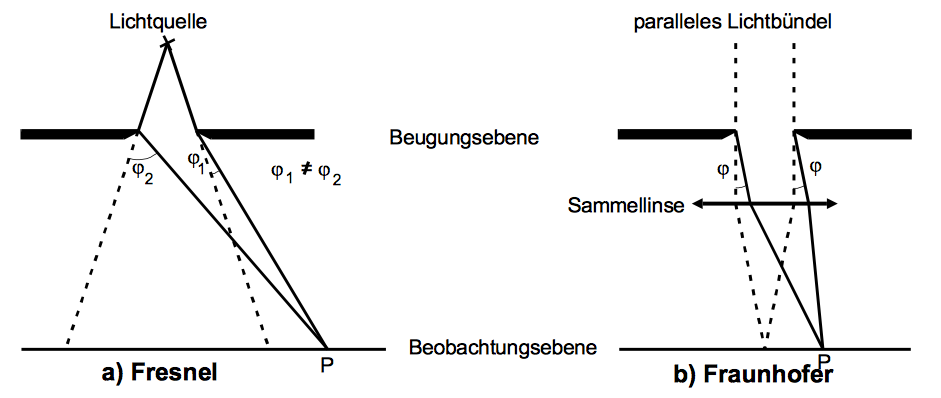
\includegraphics[width=0.8\textwidth]{bilder/FresUndFrau.png}
  \caption{Fresnel- und Fraunhoferbeugung am Einzelspalt \cite{406}}
  \label{fig:FresUndFrau}
\end{figure}
Bei der Fresnelbeugung liegen Lichtquelle und Beobachtungspunkt $P$ im Endlichen.
Das führt dazu, dass die Strahlen, die in $P$ interferieren, unterschiedliche Winkel
$\varphi$ haben. Das Strahlenbündel ist divergent. Bei der Fraunhoferbeugung liegen jedoch
Lichtquelle und Beobachtungspunkt
beide im Unendlichen, was dazu führt, dass die Winkel $\varphi$ gleich sind.
Um $P$ ins Unendliche zu bekommen, wird eine Sammellinse verwendet, welche
das Lichtbündel in die Brennebene abbildet.
Somit ist das Strahlenbündel parallel und es herrscht eine ebene Wellenfront.
Aus mathematischen Gründen wird nun nur noch auf die Fraunhoferbeugung eingegangen.

Ist die Länge eines Spaltes groß gegenüber seiner Breite $b$, so wird das Lichtbündel
in nur einer Dimension (hier X-Koordinate) begrenzt. Die Feldstärke einer
ebenen Welle lautet
\begin{equation}
  A(z,t) = A_0 \exp{(i(\omega t - 2\pi z / \lambda))}
\end{equation}
bei Ausbreitung in Z-Richtung, pro Längeneinheit. Ein paralleles Lichtbündel wird
erreicht, indem in Laser in einer Entfernung aufgestellt wird, die groß im
Vergleich zur Spaltbreite $b$ ist.

\subsection{Beugungserscheinung}
Die Beugung kann mithilfer des Huygens-Fresnel-Prinzips erklärt werden. Dies besagt,
dass jeder Punkt der Wellenfront Elementarwellen in Form von Kugelwellen aussendet,
welche miteinander interferieren und so ein Wellenfront bilden, die gleich der
Einhüllenden der Elementarwellen ist. Der Schwingungszustand eines beliebigen Punktes
im Wellenfeld ergibt sich durch die Überlagerung sämtlicher Elementarwellen, die
zum selben Zeitpunkt in dem betrachteten Punkt ankommen. Die Strahlenbündel einer
Wellenfront stellen dabei infinitesimal kleine Ausschnitte einer Kugelwelle dar,
deren Normalen in $\varphi$ - Richtung zeigen.
Abb. \ref{fig:Fraunhofer} zeigt die Fraunhoferbeugung, wenn man die Strahlenbündel
einzeln betrachtet.
\begin{figure}
  \centering
  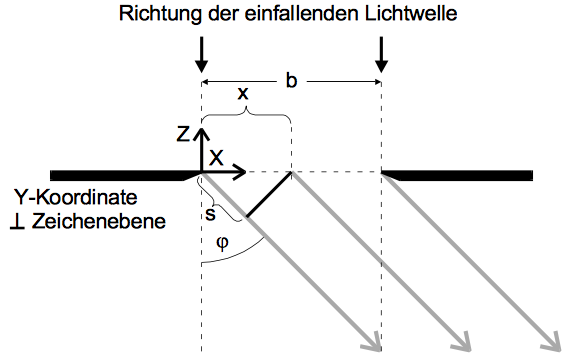
\includegraphics[width=0.5\textwidth]{bilder/Fraunhofer.png}
  \caption{Teilstrahlen der Fraunhoferbeugung \cite{406}}
  \label{fig:Fraunhofer}
\end{figure}
Die Phasendifferenz $\delta$ zwischen zwei Strahlenbündeln mit dem Abstand $x$
und dem Wegunterschied $s$ ergibt sich aus
\begin{equation}
  \delta = \frac{2 \pi s}{\lambda} = \frac{2 \pi x \sin{(\varphi)}}{\lambda}.
\end{equation}
Zur Berechnung der Amplitude $B$, die in Richtung $\varphi$ zeigt, muss über
alle Strahlenbündel von sämtlichen Punkten in der Spaltöffnung summiert werden.
Aufgrund der infinitesimal kleinen Breite $dx$ ergibt sich daraus das Integral
\begin{align}
  B(z,t,\varphi) &= A_0 \int_0^b \exp{\Bigg(i\bigg(\omega t - \frac{2 \pi z}{\lambda}
  + \delta \bigg)\Bigg)}dx \\
  &= A_0 \exp{\Bigg(i \bigg( \omega t - \frac{2\pi z}{\lambda}\bigg)\Bigg)}
  \int_0^b \exp{\bigg(\frac{2 \pi i x \sin{(\varphi)}}{\lambda}\bigg)}dx.
\end{align}
Nach dem Integrieren und verschiedenen Umformungen folgt dann:
\begin{equation}
  B(z,t,\varphi) = A_0 \exp{\Bigg(i \bigg( \omega t - \frac{2\pi z}{\lambda}\bigg)\Bigg)}
  \cdot \exp{\bigg(\frac{\pi i b \sin{(\varphi)}}{\lambda} \bigg)} \cdot
  \frac{\lambda}{\pi \sin{(\varphi)}} \sin{\bigg(\frac{\pi b \sin{(\varphi)}}{\lambda}\bigg)}.
  \label{eqn:Amplitude}
\end{equation}
Die Exponentialfunktionen in \eqref{eqn:Amplitude} stellen Phasenfunktionen dar.
Die erste beschreibt die Zeit- und Ortsabhängigkeit der Amplitude in Ausbreitungsrichtung
der Welle und die zweite stellt einen richtungsabhängigen Phasenfaktor dar, der
die Intensitätsmessung nicht beeinträchtigt.
Mit der Abkürzung
\begin{equation}
  \eta = \frac{\pi b \sin{(\varphi)}}{\lambda}
\end{equation}
wird hier nur der Faktor
\begin{equation}
  B(\varphi) = A_0 b \frac{\sin{(\eta)}}{\eta} \label{eqn:B}
\end{equation}
für die experimentelle Überprüfung benötigt.
Die Funktion \eqref{eqn:B} ist beispielhaft in Abb. \ref{fig:Amplitude} zu sehen.
\begin{figure}
  \centering
  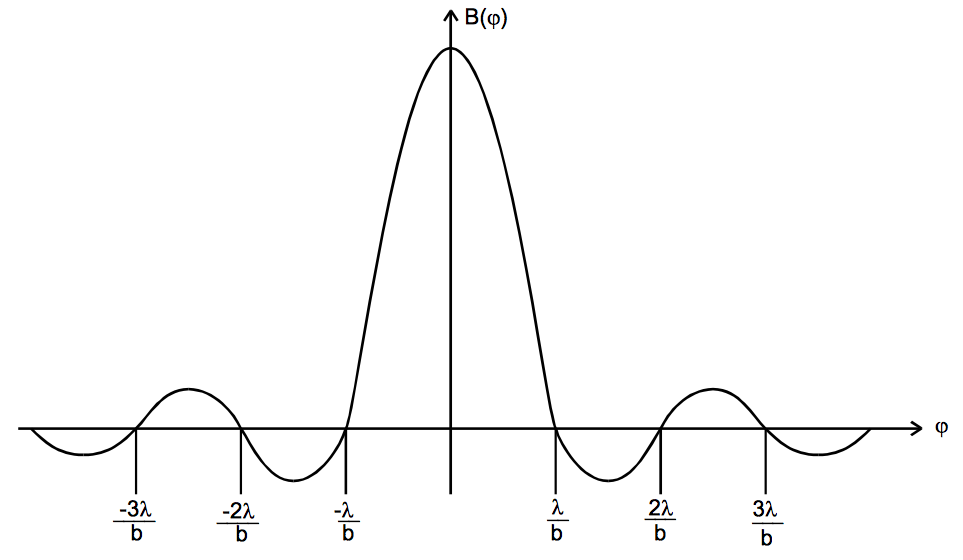
\includegraphics[width=0.6\textwidth]{bilder/Amplitude.png}
  \caption{Amplitude einer ebenen Welle am Parallelspalt \cite{406}}
  \label{fig:Amplitude}
\end{figure}
Die Nullstellen dieser Funktion liegen bei
\begin{equation*}
  \sin{(\varphi_\su{n})} = \pm n \frac{\lambda}{b}
\end{equation*}
mit $n = 1, 2, 3,..$.

Zur Bestimmung der Intesität $I(\varphi)$ muss das zeitliche Mittel betrachtet
werden, da die hohen Lichtfrequenzen von $\omega = 10^{14}\Hz$ bis $\omega = 10^{15}\Hz$
eine direkte Messung unmöglich machen. Für $I(\varphi)$ am Parallelspalt gilt
\begin{equation}
  I(\varphi) \propto B(\varphi)^2 = A_0^2b^2 \bigg(\frac{\lambda}{\pi b \sin{(\varphi)}}\bigg)
  \cdot \sin^2{\bigg(\frac{\pi b \sin{(\varphi)}}{\lambda}\bigg)}.
  \label{eqn:Intensität}
\end{equation}
Die Beugungsfigur aus \eqref{eqn:Intensität} weist Minima auf, wenn die
Amplitudenfunktion \eqref{eqn:Amplitude} Nullstellen hat. Die Höhe der Maxima
nimmt näherungsweise mit $\varphi^2$ ab.
